%! TeX program = xelatex
\documentclass[crop]{standalone}
\usepackage{amsmath,amssymb,mathrsfs}
\usepackage{tikz}
\usepackage{tikz-cd}
\usetikzlibrary{babel}

\usepackage{fontspec}

\begin{document}
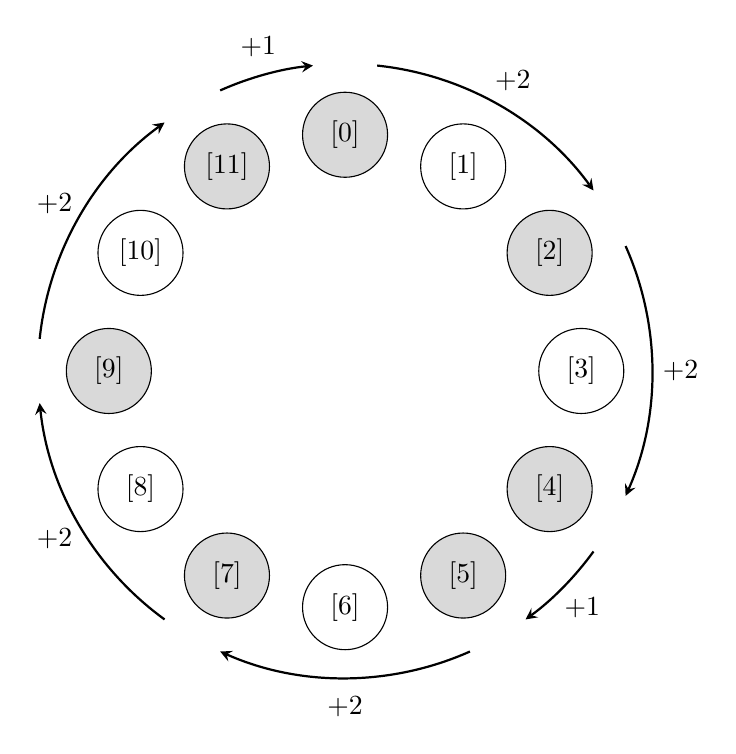
\begin{tikzpicture}[scale=3,>=stealth]

% PARAMETERS
\def\R{1}           % radius of nodes
\def\r{0.18}        % small circle radius
\def\Rm{1.3}        % radius for arrows
\def\gap{6}         % degrees to leave at start/end of arc

% Gray-filled nodes
\def\graylist{{0,2,4,5,7,9,11}}

% -------------------------
% Draw nodes
\foreach \i in {0,...,11}{
    \pgfmathsetmacro{\ang}{90 - 360/12*\i}
    \coordinate (P\i) at (\ang:\R);

    \ifnum\i=0 \def\col{gray!30} \else
    \ifnum\i=2 \def\col{gray!30} \else
    \ifnum\i=4 \def\col{gray!30} \else
    \ifnum\i=5 \def\col{gray!30} \else
    \ifnum\i=7 \def\col{gray!30} \else
    \ifnum\i=9 \def\col{gray!30} \else
    \ifnum\i=11 \def\col{gray!30} \else
        \def\col{white}%
    \fi\fi\fi\fi\fi\fi\fi
    \draw[fill=\col] (P\i) circle (\r);
    \node at (P\i) {[\i]};
}

% -------------------------
% Draw arrows (clockwise, gaps applied)
% Hard-coded start/end angles (degrees)
\def\arrow#1#2#3{%
    % start and end angles
    \pgfmathsetmacro{\angStart}{90 - 360/12*#1 - \gap} % clockwise
    \pgfmathsetmacro{\angEnd}{90 - 360/12*#2 + \gap} 
    % if end < start, add 360 to go clockwise
    \ifdim \angEnd pt>\angStart pt
        \pgfmathsetmacro{\angEnd}{\angEnd-360}
    \fi
    \draw[->, thick] (\angStart:\Rm) arc[start angle=\angStart, end angle=\angEnd, radius=\Rm];
    % midpoint for label
    \pgfmathsetmacro{\midang}{(\angStart+\angEnd)/2}
    \node at (\midang:\Rm+0.12) {#3};
}

% Sequence 0→2→4→5→7→9→11→0
\arrow{0}{2}{+2}
\arrow{2}{4}{+2}
\arrow{4}{5}{+1}
\arrow{5}{7}{+2}
\arrow{7}{9}{+2}
\arrow{9}{11}{+2}
\arrow{11}{0}{+1} % last arrow handled

\end{tikzpicture}

\end{document}
